\begin{figure}[H]
\centering
\includegraphics[page=6,width=0.48\textwidth]{\FCNCFigures/xTFW/showFake/NOMINAL/reg2mtau1b2jos_vetobtagwp70_highmet/tau_pt_0.pdf}
\put(-100, 140){\textbf{(a1)}}
%\put(-120, 130){\footnotesize{$t_h\thadhad$-2j (OS)}}
\includegraphics[page=6,width=0.48\textwidth]{\FCNCFigures/xTFW/showFake/NOMINAL/reg2mtau1b3jos_vetobtagwp70_highmet/tau_pt_0.pdf}
\put(-100, 140){\textbf{(b1)}}
%\put(-120, 130){\footnotesize{$t_h\thadhad$-3j (OS)}}

\includegraphics[page=6,width=0.48\textwidth]{\FCNCFigures/xTFW/showFake_samesign/reg2mtau1b2jos_vetobtagwp70_highmet/tau_pt_0.pdf}
\put(-100, 140){\textbf{(a2)}}
%\put(-120, 130){\footnotesize{$t_h\thadhad$-2j (OS)}}
\includegraphics[page=6,width=0.48\textwidth]{\FCNCFigures/xTFW/showFake_samesign/reg2mtau1b3jos_vetobtagwp70_highmet/tau_pt_0.pdf}
\put(-100, 140){\textbf{(b2)}}
%\put(-120, 130){\footnotesize{$t_h\thadhad$-3j (OS)}}

\includegraphics[page=6,width=0.48\textwidth]{\FCNCFigures/xTFW/showFake_sideband/reg2mtau1b2jos_vetobtagwp70_highmet/tau_pt_0.pdf}
\put(-100, 140){\textbf{(a3)}}
%\put(-120, 130){\footnotesize{$t_h\thadhad$-2j (OS)}}
\includegraphics[page=6,width=0.48\textwidth]{\FCNCFigures/xTFW/showFake_sideband/reg2mtau1b3jos_vetobtagwp70_highmet/tau_pt_0.pdf}
\put(-100, 140){\textbf{(b3)}}
%\put(-120, 130){\footnotesize{$t_h\thadhad$-3j (OS)}}
\caption{ The distributions of $\tau$ $\pt$ in the $t_h\thadhad$-2j (SS)(a1-3), $t_h	hadhad$-2j (OS) (b1-3), using the nominal (1), SS CR derived (2), OS CR derived FFs. }
\label{fig:fakeEstimation_had}
\end{figure}

